\documentclass[12pt]{exam}

\usepackage{amsmath}

\usepackage{times}
\usepackage{helvet}
\usepackage{courier}

%\usepackage{fontspec}
%\setmainfont{Liberation Serif}
%\setsansfont{Liberation Sans}

\usepackage{geometry}
\geometry{               
	letterpaper,
	bottom=0.5in,
	top=0.5in,
	left=0.5in,
	right=0.5in,
        footskip=2ex
}

\usepackage{graphicx}

\usepackage{titling}
\pretitle{\begin{center}\LARGE\sffamily}
\posttitle{\par\end{center}\vspace{-4ex}}
\preauthor{\begin{center}\large\sffamily}
\postauthor{\par\end{center}\vspace{-12ex}}
\setlength{\droptitle}{-60pt}

\usepackage{multienum}

%\usepackage{fancyhdr}
%\pagestyle{fancy}

%\fancyhf{}
%\renewcommand{\headrule}{}
%\fancyfoot[C]{\thepage}

\usepackage{multicol}
\setlength{\columnseprule}{0.5pt}

\setlength{\parindent}{0pt}


\begin{document}

\begin{center}
  {\Large\sffamily Final Exam} \\
  {\large\sffamily Foundations of College Algebra}
\end{center}
\begin{flushright}
Name:\underline{\hspace{2.5in}}
\end{flushright}

\textbf{Directions:} Answer the questions below.
You are allowed to use a calculator, but not notes, a cell phone, or smart watch.
Each question is worth 5 points.

\begin{questions}
\question[5] Simplify. $$\sqrt{64}\div\sqrt{16}+3^2 \cdot 2-17$$ \vspace\fill
\question[5] Find the prime factorization of the following number. Write any repeated factors using exponents. $$684$$ \vspace\fill
\question[5] Multiply. Write the answer in simplest form. $$1 \frac34\cdot \frac4{21}$$ \vspace\fill
\question[5] Divide. Write your answer in simplest form. $$ \frac3{55} \div \frac{6}{77}$$ \vspace\fill
\question[5] Add and simplify. $$\frac3{99} + \frac3{22}$$ \vspace\fill \pagebreak
\question[5] A landscape architect is planning a border for a flower garden shaped like a triangle.
The sides of the garden measure 16.2 feet, 24.66 feed, and 22.8 feet. Find the amount of border material needed.\\
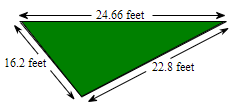
\includegraphics[height=1.5in]{FinalTriangle.png}
\question[5] A self-tanning lotion advertises that a 3-oz bottle will provide six applications.
Jen found a great deal on a 14-oz bottle of the self-tanning lotion she had been using.
Based on advertising claims, how many applications of the self-tanner should Jen expect?\vspace\fill
\question[5] In 1999, total revenue of a music company from music sales and licensing was \$14.9 billion. It was forecasted that this number would continue to drop until it reached \$5.5 billion in 2014. Find this percent decrease in music revenue.\vspace\fill
\question[5] The sales tax is \$141.30 on a stereo system purchase of \$1570. Find the sales tax rate. \vspace\fill
\question[5] Sketch the right triangle and find the length of the side not given.
(Each length is in units.)
$$\text{leg}=17 \text{, leg}=23$$ \vspace\fill \pagebreak
\question[5] Decide whether the given number is a solution of the given equation. $$ \frac{x}7 - 3 = -2; \qquad x=35$$ \vspace\fill
\question[5] Solve the equation. $$-6(n-2)=8-5n$$ \vspace\fill
\question[5] Solve the equation. $$x+6=3x+16$$ \vspace\fill
\question[5] Solve the equation for $x$. $$ \frac34 x - \frac12=-2$$ \vspace\fill \pagebreak
\question[5] Solve the inequality. Write your answer in set notation. $$7(x+1)-6x\geq-8$$ \vspace\fill
\question[5] Graph the linear equation. $x+3=0$ \\
  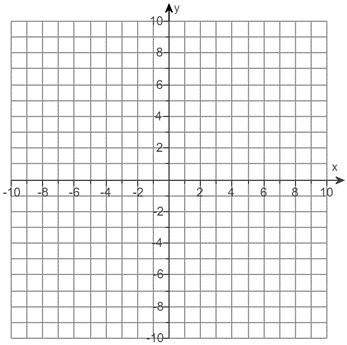
\includegraphics[height=3in]{GraphPaper.png}
\question[5] Write an equation of the line with the given slope, $m$, and $y$-intercept $(0,b)$. $$ m=-\frac34 \text{, } b=\frac25$$ \vspace\fill
\question[5] Use the product rule to simplify the expression. Write the results using exponents. $$(3z^{11} )(-2z^6)(z^2 )$$ \vspace\fill \pagebreak
\question[5] Subtract. $$(5z^2-9z+9)-(10z^2+3z-7)$$ \vspace\fill
\question[5] Multiply using the FOIL method. $$(y^2+9)(5y+7)$$ \vspace\fill
\question[5] Factor the trinomial completely. $$x^2-2x-24$$ \vspace\fill
\question[5] Solve the equation. $$x^2-7x+12=0$$ \vspace\fill
\end{questions}

\end{document}
